\section{1962: 1st Reduced Instruction Set Computer}
From 1950 to 1970 the National Laboratories promoting the development of atomic
weapons (Los Alamos, Livermore) came up with insatiable demands of computing power.
Their calls for faster computers presented massive challenges to computer designers,
and their financial resources promised enormous challenges. The goal was, simply
speaking, to develop a super-computer.

The company that first picked up the challenge was CDC (Control Data Corporation,
Minneapolis), and its chief designer Seymour Cray. After the CDC 1604, he undertook
a radical departure from the ongoing trend, which had led to computers with more and
more complicated and large instruction sets. His idea was to provide only a few,
basic instructions, all executable with greatest speed. Apart from this, he relied on
the new component family with ECL (emitter-coupled logic) technology, which provided
very fast transistors, but with the disadvantage of requiring large amounts of current
(energy). As a consequence, his main challenge became not designing logic, but cooling
the heated transistors. This computer was built before integrated circuits (chips) had
become available.

The CDC 6000 architecture is briefly sketched as follows. The memory consists of
262144 ($=2^{18}$) 60-bit words, and the processor contains 3 sets of 8 registers.
The data registers XO - X7 are 60 bits wide, the address registers AO - A7, and the
index registers BO - B7 are 18 bits wide. Instructions are either 15 or 30 bits long,
2, 3, or 4 fitting into a 60-bit word.
\begin{figure}[h!]
  \centering
  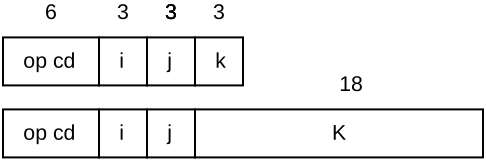
\includegraphics[width=.5\textwidth]{i/2}
\end{figure}
examples:
\begin{verbatim}
  Bi := Bj + Bk
  Ai := Bj + K
\end{verbatim}

The computer used 1-complement representation of integers. This allowed faster
sign inversion, but provided 2 forms for zero, giving rise to several unpleasant
problems.

A clever oddity is the rule that assignments to an A-register have a side-effect on
the corresponding X-register. Assigning an address to an A-register was the only way
to transfer data from and to memory. (This "feature" was loved by compiler builders).
\begin{verbatim}
  Ai := a -> Xi := mem[a] for i< 6 load
  Ai := a -> mem[a] := Xi for i>=6 store
\end{verbatim}
